\documentclass[a4paper, 10pt, final, garamond]{book}
\usepackage{cours-preambule}
\graphicspath{{./figures/}}
\addto\captionsfrench{\renewcommand{\figurename}{Fig.}}

\makeatletter
\renewcommand{\@chapapp}{Contr\^ole de connaissances}
\makeatother

% \toggletrue{student}
% \toggletrue{corrige}
\renewcommand{\mycol}{black}
% \renewcommand{\mycol}{gray}

\hfuzz=5.003pt

\begin{document}
\setcounter{chapter}{4}

\settype{enon}
\settype{solu}

\chapter{Électrocinétique~: premier ordre et harmonique\ifstudent{~(15')}}

\begin{enumerate}[label=\sqenumi, leftmargin=10pt]
	\item[n]{13}%
	      \noindent
	      \begin{minipage}[t]{.69\linewidth}
		      On suppose le circuit LC série suivant, en régime libre. On suppose le
		      condensateur initialement chargé à la tension $E$, et on ferme
		      l'interupteur à $t=0$. Déterminer l'équation différentielle sous forme
		      canonique de $u_C$ pour $t \geq 0$, donner les conditions initiales et
		      comment les déterminer, et résoudre l'équation différentielle pour
		      trouver $u_C(t)$ \textbf{et} $i(t)$.
	      \end{minipage}
	      \hfill
	      \begin{minipage}[t]{.29\linewidth}
		      ~
		      \vspace{-35pt}
		      \begin{center}
			      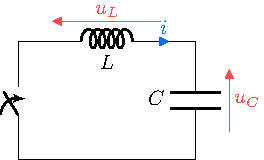
\includegraphics[width=.8\linewidth]{lc_descendant-intens}
			      \captionof{figure}{}
		      \end{center}
	      \end{minipage}
	      \begin{isd}[sidebyside align=top]
		      \vspace{-15pt}
		      \psw{%
			      \begin{DispWithArrows*}[fleqn, mathindent=4em]
				      u_L + u_C &\stm{=} 0
				      \Arrow{$u_L \stm{=} L \dv{i}{t}$\\ et $i = C \dv{u_C}{t}$}
				      \\\Lra
				      LC \dv[2]{u_C}{t} + u_C &= 0
				      \Arrow{forme canonique\\et $\w_0 = \frac{1}{\sqrt{LC}} \pt{1}$}
				      \\
				      \Lra \dv[2]{u_C}{t} + \w_0{}^2 u_C &\stm{=} 0
			      \end{DispWithArrows*}
			      On injecte la forme générique de solution~:
			      \[
				      u_C(t) \stm{=} K \exr^{rt}
				      \Ra
				      r^2 \times \cancel{K \exr^{rt}} + \w_0{}^2\cancel{K\exr^{rt}} = 0
				      \Lra
				      r_{\pm} \stm{=} \pm \jw_0
			      \]
			      D'où la forme générale~:
			      \[
				      u_C(t) \stm{=} A\cos(\w_0 t) + B\sin(\w_0 t)
			      \]
			      Or, $u_C(0^-) = E = u_C(0^+)$ et $i(0^-) = 0 = i(0^+)$ par
			      continuité de
			      $u_C(t)$ aux bornes de $C$ et de $i(t)$ traversant la bobine \pt{1}.
		      }%
		      \tcblower
		      \psw{%
			      On trouve $A$ avec la première condition initiale~:
			      \[
				      u_C(0) = A\cos(0) + B\sin(0)
				      \Lra
				      \boxed{A = E}
				      \hspace{12pt} \pt{1}
			      \]
			      On trouve $B$ avec la seconde condition initiale~:
			      \begin{gather*}
				      \dv{u_C}{t} = -A\w_0\sin(\w_0t) + B\w_0\cos(\w_0t)
				      \Ra
				      \qty(\dv{u_C}{t})_0 \stm{=} B\w_0
				      \\
				      \text{et} \quad
				      i(0) = 0 = C \qty(\dv{u_C}{t})_0 = CB\w_0
				      \quad \Ra
				      \boxed{B = 0}
				      \hspace{12pt} \pt{1}
			      \end{gather*}
			      D'où
			      \[
				      \boxed{u_C(t) = E\cos(\w_0t)} \pt{1}
			      \]
			      On obtient ensuite $i$ avec la relation courant-tension~:
			      \[
				      \boxed{i(t) = C \dv{u_c}{t} \stm{=} -CE \w_0 \sin(\w_0t)}
			      \]
		      }%
		      \vspace{-15pt}
	      \end{isd}
	      \vspace*{\fill}
	\item[n]{7}%
	      Faire un bilan de puissance pour le circuit LC libre, et montrer que
	      l'énergie totale est conservée à chaque instant. Tracer $\Ec_C$, $\Ec_L$
	      et $\Ec_{\tot}$.
	      \smallbreak
	      \begin{isd}[righthand ratio=.25]
		      \psw{%
			      \vspace{-15pt}
			      \begin{DispWithArrows*}
				      u_Ci + u_Li &\stm{=} 0
				      \Arrow{$i = C \dv{u_C}{t}$\\et $u_L = L \dv{i}{t}$}
				      \\
				      \Lra
				      u_C\times C \dv{u_C}{t} + L \dv{i}{t}\times i &= 0
				      \Arrow{$f \times f' \stm{=} \left( \frac{1}{2}f^{2} \right)'$}
				      \\\Lra
				      \dv{}{t} \Big(
				      \underbracket[1pt]{\frac{1}{2}Cu_C{}^2}_{=\Ec_C \pt{1}} +
				      \underbracket[1pt]{\frac{1}{2}Li^2}_{=\Ec_L \pt{1}}
				      \Big) &= 0
				      \Arrow{$\Ec_{\tot} = \Ec_C + \Ec_L$}
				      \\\Lra
				      \Aboxed{\dv{\Ec_{\tot}}{t} \stm{=} 0}
			      \end{DispWithArrows*}
			      \vspace{-15pt}
		      }%
		      \tcblower
		      \begin{center}
			      \sswitch{%
				      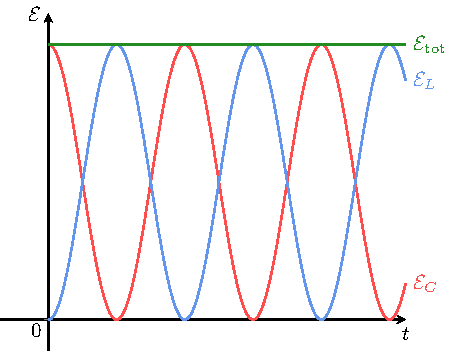
\includegraphics[width=\linewidth,
					      draft=true]{carac-lc_descendant-bilan}
			      }{%
				      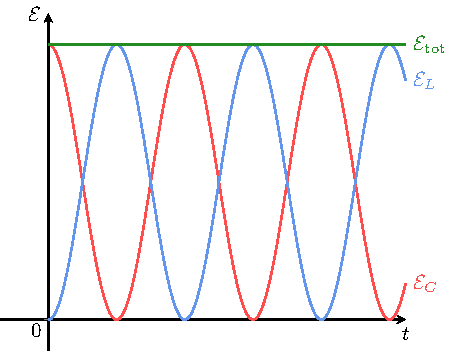
\includegraphics[width=\linewidth]{carac-lc_descendant-bilan}
			      }%
			      \vspace{-15pt}
			      \captionof{figure}{\protect\pt{1}\psw{+}\protect\pt{1}}
		      \end{center}
	      \end{isd}
	      \vspace*{\fill}
	      % \item[n]{4}%
	      % Tracer les solutions $u_C(t)$ et $i(t)$ dans l'\textbf{espace des
	      % phases} (axe $x = u_C(t)$, axe $y = i(t)$), et \textbf{indiquer le
	      % sens
	      % de parcours}. Expliquer succinctement pourquoi on obtient cette forme.
	      % \smallbreak
	      % \begin{isd}[lefthand ratio=.25]
	      % \begin{center}
	      % \sswitch{%
	      % 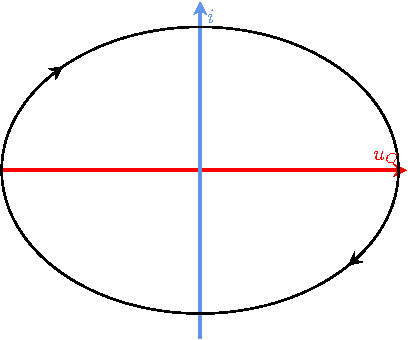
\includegraphics[width=\linewidth, draft=true]{carac-rlc_xy-harmo}
	      % }{%
	      % 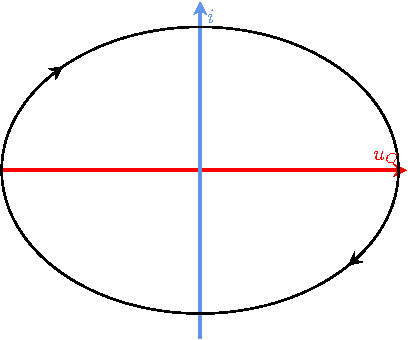
\includegraphics[width=\linewidth]{carac-rlc_xy-harmo}
	      % }%
	      % \vspace*{-20pt}
	      % \captionof{figure}{\protect\pt{1}\psw{+}\protect\pt{1}}
	      % \end{center}
	      % \tcblower
	      % \psw{%
	      % On obtient une ellipse étant donné que $u_C(t) \propto \cos(\w_0t)$
	      % et que $i(t) \propto \sin(\w_0t)$ \pt{1}.
	      % \smallbreak
	      % Par construction, cela correspond à tracer un cercle déformé (donc
	      % une ellipse) puisque $\cos^{2}(x) + \sin^{2}(x) = 1$. \pt{1}
	      % }%
	      % \vspace*{-15pt}
	      % \end{isd}
	\item[n]{+2}%
	      Explain the \textsc{Peltier} effect in your own words.
	      \smallbreak
	      \psw{%
		      At the junction between two different metals, electrons can gain or
		      lose heat because of the increased or reduced electrical potential
		      energy levels between them. Thus, applying a current creates a
		      difference in temperature between the metals.
	      }%
\end{enumerate}

\ifstudent{%
	\begin{tikzpicture}[remember picture, overlay]
		\node[anchor=north west, align=left]
		at ([shift={(1.4cm,0)}]current page.north west)
		{\\[5pt]\Large\bfseries Nom~:\\[10pt]\Large\bfseries Prénom~:};
		\node[anchor=north east, align=right]
		at ([shift={(-1.5cm,-17pt)}]current page.north east)
		{\Large\bfseries Note~:\hspace{1cm}/20};
	\end{tikzpicture}
}%

\end{document}
